\lecture{25}{2024-12-10}{corps $\mathbb{F}_4$}{}

\begin{parag}{La multiplication dans $\mathbb{F}_4$}
    
        Pour ne pas confondre l'indéterminée $t$ des polynômes et l'élément $t$ donné comme reste de division, on choisit d'appeler $\alpha$ le reste $t$ ou plus précisément la classe $[t]$ de $t$ dans "\textit{l'anneau des polynôme $\mathbb{F}_2[t]$ modulo $t^2 + t + 1$}"
        \begin{enumerate}
            \item Comme \textcolor{red}{ensemble} $\mathbb{F}_4 = \{0, 1, \alpha, \alpha + 1\}$
            \item \textcolor{red}{l'addition} est celle des polynômes, chaque éléments est son propres opposé.
            \item la \textcolor{red}{multiplication} est celle des polynôme, modulo $t^2 + t + 1$, en particulier $\alpha^2 = \alpha + 1$. On a donc aussi $\mathbb{F}_4 = \{0, 1, \alpha, \alpha^2\}$   
        \end{enumerate}
        On peut par exemple prendre $\alpha \cdot \alpha^2 = \alpha^3 = 1$
        \begin{framedremark}
            Ici on a choisi $t^2 + t + 1$ pour pouvoir construire nos calcul, mais le critère pour choisir est que c'est un polynôme dans $\mathbb{F}_2$ avec des coefficient irréductible
        \end{framedremark}
        \begin{subparag}{Le polynôme $t^2 + t + 1 \in \mathbb{F}_4[t]$}
            Le polynôme $p(t) = t^2 + t + 1 \in \mathbb{F}_2[t]$ est irréductible, mais on peut aussi le voir comme un polynôme de $\mathbb{F}_4[t]$, car ses coefficients sont dans $\mathbb{F}_2 \subset \mathbb{F}_4$.
            \\
            Calculons $p(\alpha)$
            \[p(\alpha) = \alpha^2 + \alpha + 1 = \begin{cases}
                \alpha + 1  + \alpha + 1 = 2\alpha + 2  = 0\\
                [t]^2 + [t] + 1  = [t^2 + t + 1] = 0
            \end{cases}\]
            le deuxième cas est juste par la définition de $+$ et $\cdot $ dans $\mathbb{F}_4$\\
            Donc, $t-\alpha = t + \alpha$ divise $t^2 + t + 1$ dans $\mathbb{F}_4$. Effectuons la divisions euclidienne.
            
                \begin{center}
        \begin{tabular}{c@{\,}c@{\,}c@{\,}c@{\,}c@{\,}c@{\,}c@{\,}c@{\,}|l}
            $t^2$ & $+$  &  $t$  &  $+$ & $1$   &   &    & $\quad$ & $t + \alpha$ \\
            \hhline{~~~~~~~~|-}
             & $t^2$ & $+$ & $\alpha t$  &    &   &    &   & $t + (\alpha + 1)$ \\
            \hhline{~-----~~|~}
              &  $(\alpha$ &  $+$ & $1)t$  & $+$   & 1  &   &   & \\
              &  $(\alpha$ & + & $1)t$ & $+$ &$\alpha(\alpha$   &  $+$  & $1)$  & \\
            \hhline{~-------|~}
              &   &    &   &  &   &    & $0$  & 
              
        \end{tabular}
        \end{center}
        \textit{PS.( j'ai galéré à faire ça sur latex donc profitez un peu)}
            
            On obtient $t^2 + t + 1 = (t+\alpha)(t + \alpha + 1)$
        \end{subparag}
        \end{parag}

        \begin{parag}{Régression linéaire : Objectif}
            On se donne un "\textit{nuage}" de points dans le plan, donnés par leurs ordonnées ($x_1, y_1), \dots, (x_n, y_n)$ et on aimerait trouver la droite qui donne la meilleures approximation :
            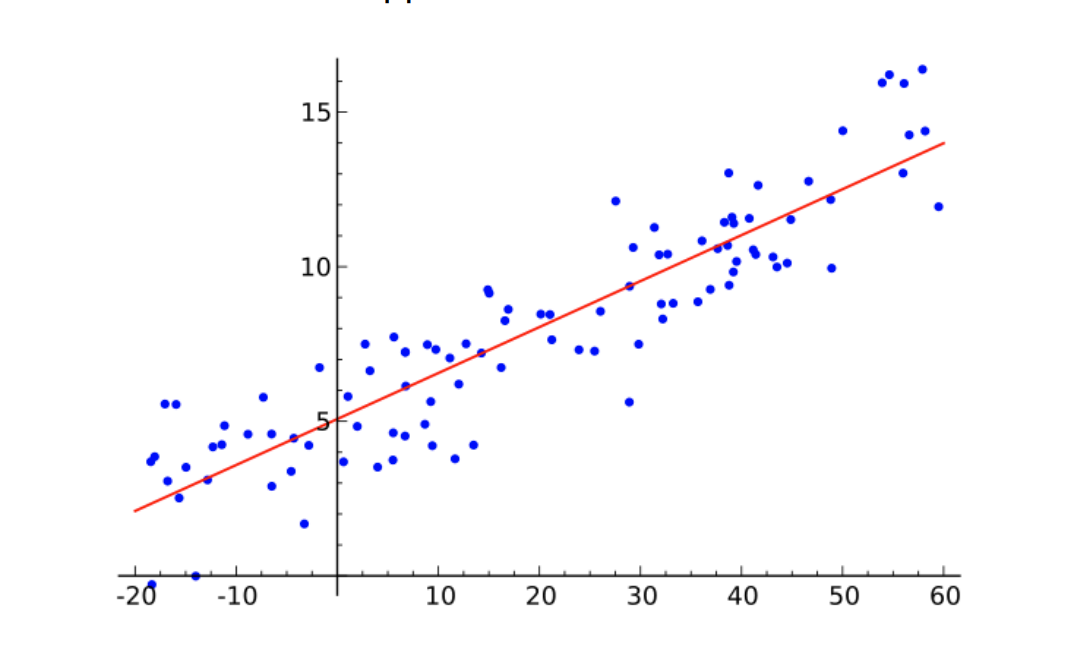
\includegraphics[scale=0.3]{Algèbre linéàaire/Screenshot 2024-12-10 153727.png}
            On cherche la droite d'équation $y = at + b$ la plus proche des points $(x_1, y_1)\dots (x_n, y_n)$ dans le sens où les distances verticales entre les point et la droite sont minimisées (voici un exemple tié de UC Buisness Analytics R programming Guide)
            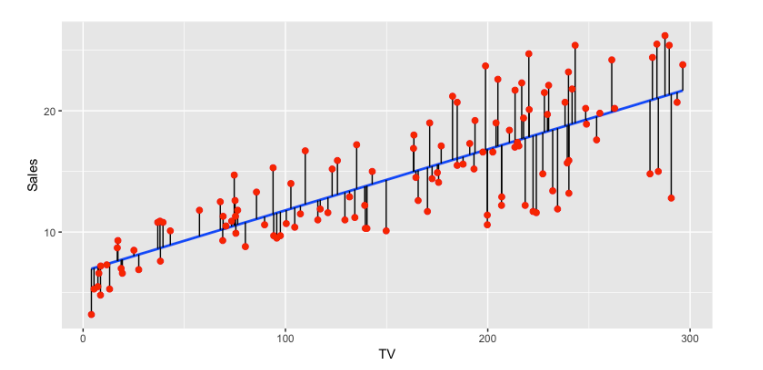
\includegraphics[scale = 0.5]{Algèbre linéàaire/Screenshot 2024-12-10 153930.png}
        \end{parag}
        \begin{parag}{Forme Matricielle}
            On écrit le système ci-dessus sous forme matricielle 
            \[\begin{pmatrix}
                x_1  & 1 \\ \vdots & \vdots \\ x_n & 1
            \end{pmatrix}\begin{pmatrix}
                a \\ b
            \end{pmatrix} = \begin{pmatrix}
                y_1 \\ \vdots \\ y_n
            \end{pmatrix}\]
            et on utilise l'équation normale pour résoudre 
            \[\begin{pmatrix}
                \sum (x_i^2 & \sum x_i\\
                \sum x_i & n
            \end{pmatrix}\begin{pmatrix}
                \hat{a}\\ \hat{b}
            \end{pmatrix} ) \begin{pmatrix}
                \sum x_iy_i \\ \sum y_i
            \end{pmatrix}\]
            \begin{subparag}{exemple}
                On cherche la droite de régression linéaire pour les points $(-2, -1), (0, 1), (2, -2), (4, 1)$
                \[A  = \begin{pmatrix}
                    -2 & 1 \\ 0 & 1 \\ 2 & 1 \\ 4 & 1
                \end{pmatrix} \; \; \; \vec{b} = \begin{pmatrix}
                    -1 \\ 1 \\-2\\ 1
                \end{pmatrix} \; \; \; \; A^T A= \begin{pmatrix}
                    24 & 4 \\ 4 & 4
                \end{pmatrix}\]
                \begin{align*}
                    A^T \vec{b} = \begin{pmatrix}
                        2 \\ -1
                    \end{pmatrix}
                \end{align*}
                On doit résoudre le système $A^TA \cdot \hat{a} = \hat{b} $
                Ce qui nous donne
                $\left(
                \begin{array}{cc|c}
                    24 &4 & 2  \\
                     4&4 & -1 
                \end{array}\right) \to \left(
                \begin{array}{cc|c}
                    1 &0 & 3/20  \\
                     0&1 & -2/5 
                \end{array}\right) $ et donc, $y = \frac{3}{20}t - \frac{2}{5}$
            \end{subparag}
            \begin{framedremark}
                la droite qu'on trouve est toujours unique, a part dans le cas ou le noyau de la matrice n'est pas nulle, et le seul moyen d'y arriver et que la matrice soit $\begin{pmatrix}
                    1 &1 \\
                    \vdots  & \vdots\\
                    1 & 1
                \end{pmatrix}$ ce qui ferait que tout les points se trouvent au même endroits.
            \end{framedremark}
        \end{parag}
        \begin{parag}{Debriefing sur le produit scalaire}
            Nous avons utilisé jusqu'ici le produit scalaire standard dans $\mathbb{R}^n$. Les propriétés du produit scalaire font que d'associer à une paire de vecteurs $\vec{u}$ et $\vec{v}$ le produit $\vec{u}\cdot \vec{v}$ est une opération linéaire en chaque variable.
            \begin{enumerate}
                \item $\vec{u}\cdot(\vec{v}+\vec{w}) = \vec{u}\cdot\vec{v} + \vec{u}\cdot\vec{w}$
                \item $\vec{u}\cdot(\alpha\vec{v}) = \alpha(\vec{u}\cdot \vec{v})$
                \item $(\vec{u}+\vec{v}) \cdot \vec{w} = \vec{u}\cdot\vec{w} + \vec{v}\cdot \vec{w}$
                \item $(\alpha\vec{u})\cdot \vec{v} = \alpha(\vec{u}\cdot\vec{v})$
            \end{enumerate}
        \end{parag}
        \begin{parag}{Formes bilinéaires}
            Ceci nous motive à introduire un nom à d'autre application de deux variable, définies en général sur un espace vectoriel arbitraire.
            \begin{deinition}
                Soit $V$ un espace vectoriel. Une \textcolor{red}{forme bilinéaire symétrique} est une application $V \times V \to \mathbb{R}$ qui associe à tout couple de vecteurs $(u, v)$ un nombre réel $\langle u, v \rangle$ tel que
                \begin{enumerate}
                    \item commutativité $\langle u, v \rangle ) \langle v, u \rangle$
                    \item distributivité $\langle u + u', v \rangle = \langle u, v \rangle + \langle u' , v \rangle$
                    \item linéairité $\langle \alpha u, v \rangle = \alpha \langle u, v \rangle$
                \end{enumerate}
                \begin{framedremark}
                    Une forme linéaire est une application linéaire $V \to \mathbb{R}$
                \end{framedremark}
            \end{deinition}
            \begin{subparag}{Exemple}
                Le produit scalaire standard de $\mathbb{R}^2$ est une forme bilinéaire symétrique.
                \\
                Il y a de nombreuse autres formes bilinéaires symétriques. Par exemple $\langle \begin{pmatrix}
                    u_1 \\ u_2,  
                \end{pmatrix}, \begin{pmatrix}
                    v_1 \\ v_2
                \end{pmatrix}\rangle = 7u_1v_1 + 2u_1v_2 + 2u_2v_1 + 4u_2v_2$
            \end{subparag}
        
        \end{parag}

        \begin{parag}{Matrices symétriques}
            \begin{subparag}{Proposition}
                \begin{theoreme}
                    On représente une forme bilinéaire symétrique sur $\mathbb{R}^n$ par une matrice symétrique $A$ carrée de taille $n \times n$.
                \end{theoreme}
            \end{subparag}
            \begin{subparag}{Preuve}
                On pose $a_{ij} = \langle e_i, e_j\rangle = \langle e_j, e_i \rangle = a_{ji}$ si bien que 
                \begin{formule}
                    \[\langle u, v \rangle  = u^TAv\]
                \end{formule}
                En effet, $u = u_1e_1 + \cdots +u_ne_n$ et $v = v_1e_1 + \cdots + v_ne_n$. Alors:
                \[\langle e, v \rangle )\sum_i \sum_j u_iv_j\langle e_i, e_j\rangle = \sum_i \sum_j u_iv_ja_{ij} = \sum_i u_i\left(\sum_j a_{ij}v_j \right)\]
                \[= \sum_i u_i(Av)_i = u^TAv\]
            \end{subparag}
            \begin{subparag}{Exemple}
                Le produit scalaire standard de $\mathbb{R}^2$ est une forme bilinéaire symétrique représentée par la matrice $I_2$
                \\
                En effet $\langle \vec{e_i}, \vec{e_j} \rangle = \delta_{ij} \begin{cases}
                    0 \text{ si } i \neq j\\
                    1 \text{ si } i =j
                \end{cases}$
                La forme bilinéaire symétrique
            \[\langle \begin{pmatrix}
                u_i \\ u_2
            \end{pmatrix}, \begin{pmatrix}
                v_1 \\ v_2
            \end{pmatrix}\rangle = 7u_1v_1 + 2u_1v_2 + 2u_2v_1 + 4u_2v_2\]
            $\langle \vec{e_1}, \vec{e_1}\rangle =\langle \begin{pmatrix}
                1 \\ 0
            \end{pmatrix}, \begin{pmatrix}
                1 \\ 0
            \end{pmatrix} \rangle = 7 \dots A = \begin{pmatrix}
                7 & 2 \\ 2 & 4
            \end{pmatrix}$
            \\
            \[\langle \begin{pmatrix}
                u_1 \\ u_2
            \end{pmatrix}, \begin{pmatrix}
                v_1 \\ v_2
            \end{pmatrix}\rangle = (u_1, u_2)\begin{pmatrix}
                7 & 2\\ 2 & 4
            \end{pmatrix}\begin{pmatrix}
                v_1 \\ v_2
            \end{pmatrix}\]
            \end{subparag}
        \end{parag}
        \begin{parag}{Espace préhilbertiens}
            Le produit scalaire euclidien défini aussi une norme :
            \[\vec{u}\cdot \vec{u} = ||\vec{u}||^2 \geq 0\]
            On arrive ici à la notion de produit scalaire dans le sens large.
            \begin{definition}
                Soit $V$ un espace vectoriel. Un \textcolor{red}{produit scalaire} est une forme bilinéaire symétrique $V \times V \to \mathbb{R}$ telle que 
                \begin{enumerate}
                    \item commutativité $\langle u, v \rangle = \langle v, u\rangle$ pour tous $u, v \in V$
                    \item distributivité $\langle u + u', v\rangle = \langle u, v \rangle + \langle u', v \rangle$ pour tout $u, u', v \in V$
                    \item linéarité $\langle \alpha u, v \rangle = \alpha \langle u, v \rangle$ pour tous $u, v \in V$ et $\alpha \in \mathbb{R}$
                    \item  $\langle u, u \rangle \geq 0$ et on a l'égalité si et seulement si $u = 0$.
                \end{enumerate}
            \end{definition}
            \begin{subparag}{Produits scalaires, exemple}
                Le produit scalaire standard de $\mathbb{R}^2$ est un produit scalaire: c'est une forme bilinéaire symétrique et $\langle \vec{u}, \vec{u}\rangle = \vec{u}^TI_2\vec{u} = u_1^2 + u_2^2 \geq 0$.
                \\
                La forme bilinéaire symétrique:
                \[\langle\begin{pmatrix}
                    u_1 \\ u_2
                \end{pmatrix}, \begin{pmatrix}
                    v_1 \\ v_2
                \end{pmatrix}\rangle = 7u_1v_1 + 2u_1v_2 + 4u_2v_2\]
                Ici
                \begin{align*}
                    
                \langle\begin{pmatrix}
                    u_1 \\ u_2
                \end{pmatrix}, \begin{pmatrix}
                    u_1 \\ u_2 
                \end{pmatrix}\rangle &= 7u_1^2 + 4u_1u_2 + 4u_2^2\\
                &= 2(u_1^2 + 2u_1u_2 + u_2^2) + 5 u_1^2 + 2u_2^2\\
                &\geq 0\\
                &= 0 \Leftrightarrow u_1 = u_2 = 0
                \end{align*}
                \begin{framedremark}
                    Exemple à avoir, 
                    $u_1v_1 - u_2v_2$ n'est pas un produit scalaire
                \end{framedremark}      
            \end{subparag}
        \end{parag}
        \begin{parag}{Exemples: polynômes et fonctions}
            Une espace vectoriel muni d'un produit scalaire est appelé \textcolor{red}{espace préhilbertien}
            \begin{enumerate}
                \item \textbf{Polynômes} dans $\mathbb{P}_n$ on pose (par exemple)
                \[\langle p, q \rangle = \int_{-1}^1 p(t)q(t) dt\]
                Ainsi $\mathbb{P}^n$ est un espace préhilbertien
                \item \textbf{Fonction réelles}. Dans $\cmath^\infty(\mathbb{R})$ on pose (par exemple)
                \[\langle f, g \rangle = \int_{-1}^1f(x)g(x)dx\]
                Ainsi $\cmath^\infty (\mathbb{R})$ est un espace préhilbertien.
            \end{enumerate}
            \begin{subparag}{Exemple}
                Dans $\mathbb{P}_2$ on pose
                \[\langle p, q\rangle = \int_{-1}^1 p(t)q(t)dt\]
                \begin{enumerate}
                    \item $\langle1, 1\rangle = \int_{-1}^11dt = 2$
                    \item $\langle1, t\rangle = \int_{-1}^1 tdt = 0$, ainsi les polynômes $1$ et $t$ sont orthogonaux
                    \item $\langle t, t\rangle = \int_{-1}^1t^2 = 2/3$
                \end{enumerate}
                Dans $\mathbb{P}_1$, ce produit scalaire est représenté par la matice
                \[\begin{pmatrix}
                    2 & 0 \\ 0 & 2/3
                \end{pmatrix}\]
                On peut continuer avec toute les autres paires possible jusqu'à pourvoir contruire la matrice de $\mathbb{P}_2$ tel que
                \[A = \begin{pmatrix}
                    2 & 0 & 2/3\\
                    0 & 2/3 & 0\\
                    2/3 & 0 & 2/5
                \end{pmatrix}\]
                Cela signifie que le produit scalaire $\langle p(t), q(t) \rangle$ se calcule en effectuant le produit matriciel
                \[(p(t))_{\cmath an}^T A(q(t))_{\cmath an}\]
                La base canonique n'est pas orthogonale. Le procédé de Gram Schmidt permet de la rendre orthogonale: $(1, t, t^2 - 1/3)$, ici $1/3$ est la projection orthogonale de $t^2$ sur $Vect\{1, t\}$
                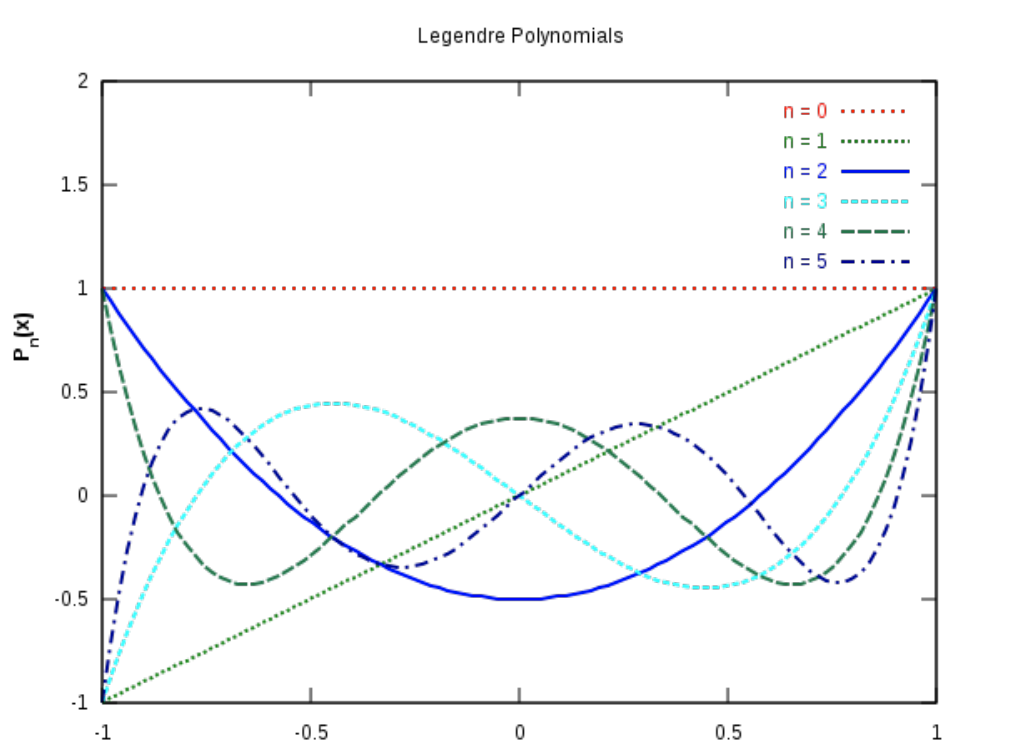
\includegraphics[scale = 0.5]{Algèbre linéàaire/Screenshot 2024-12-10 163537.png}
                
            \end{subparag}
            
        \end{parag}

        \begin{parag}{Matrice symétriques}
            \begin{definition}
                Une matrice carrée $A$ est \textcolor{red}{symétrique} si $A^T = A$
            \end{definition}
            \begin{subparag}{Exemple}
                La matrices diagonales sont symétrique, mais aussi les matrices de la forme $B^TB$ puisque le coefficient $(i, j)$ est $\vec{b_1}\cdot\vec{b_j} = \vec{b_j}\cdot \vec{b_i}$
            \end{subparag}
            \begin{theoreme}
                Soit $A$ une matrice symétrique soient $\vec{u}$ un vecteurs propre de $A$ pour la valeurs propre $\lambda$ et $\vec{v}$ un vecteurs propre de $A$ pour une autre valeurs propre $\mu$. Alors $\vec{u}$ et $\vec{v}$ sont orthogonaux
            \end{theoreme}
            \begin{subparag}{Preuve}
                On doit montrer que $\vec{u}\cdot \vec{v} = 0$.
                \\
                L'astuce est de calculer $\lambda\cdot(\vec{u}\cdot\vec{v}) \overbrace{=}^{A\vec{u} = \lambda\vec{u}} \lambda \vec{u}\cdot\vec{v} = A\vec{u}\cdot\vec{v} = (A\vec{u})^T\vec{u} = (\vec{u}^TA^T)\vec{v} = \vec{u}^T\cdot(A\vec{v}) \overbrace{=}^{déf \; \cdot} \vec{u}\cdot A\vec{v} = \vec{u}\cdot\mu\vec{v} = \mu(\vec{u}\cdot\vec{v})$ 
                \\
                Conclusion, comme $\lambda \neq \mu$, $\vec{u}\cdot\vec{v} = 0$
                \\
                \begin{framedremark}
                    \textbf{Attention}
                Si $\lambda = \mu$, ce raisonnement ne fonctionne pas, le résultat est faux en général
                \end{framedremark}
            \end{subparag}
            \begin{subparag}{Exemple}
                La matrice $A = \begin{pmatrix}
                    1 & 2\\
                    2 & 1
                \end{pmatrix}$ est symétrique. On calcule
                \[c_A(t) = (t-3)(t+1) \text{ et } E_3 = Vect\left\{\begin{pmatrix}
                    1 \\ 1
                \end{pmatrix}\right\} \text{ et } E_{-1} = Vect\left\{\begin{pmatrix}
                    -1 \\ 1
                \end{pmatrix}\right\}\]
                \\
                On sait alors par la preuve faite au dessus. que $E_3 \perp E_1$. En normalisant les vecteurs propres on obtient une base orthonormée $\bmath = \left(\begin{pmatrix}
                    \sqrt{2}/2 \\ \sqrt{2}/2
                \end{pmatrix}, \begin{pmatrix}
                    -\sqrt{2}/2 \\ \sqrt{2}/2
                \end{pmatrix}\right)$ la matrice $(Id)_\bmath^{\cmath an} = \begin{pmatrix}
                    \sqrt{2}/2 & -\sqrt{2}/2 \\
                    \sqrt{2}/2 & \sqrt{2}/2
                \end{pmatrix} = U$ est orthogonale.
                \\
                Et donc $(Id)_{\cmath an}^\bmath = U^T$ et $U^TAU = \begin{pmatrix}
                    3 & 0 \\ 0 & -1
                \end{pmatrix}$
            \end{subparag}
        \end{parag}
        \begin{parag}{Orthodiagonalisation}
            \begin{definition}
                Une matrice carrée $A$ est \textcolor{red}{diagonalisable par un changement de base orthonormée} ou \textcolor{red}{orthodiagonalisable} s'il existe une matrice $P$ orthogonale telle que $P^TAP$ est diagonale.
            \end{definition}
            \begin{theoreme}
                Une matrice $A$ est orthodiagonalisable si et seulement si elle est symétrique
            \end{theoreme}
        \end{parag}
        \begin{parag}{Théorème spectral}
            \begin{theoreme}
                Soit $A$ une matrice symétrique. Alors
                \begin{enumerate}
                    \item A admet $n$ valeurs propres réelles, compte tenu de leur multiplicité
                    \item Pour toute valeurs propres $\lambda$ on a $mult(\lambda) = \dim E_\lambda$
                    \item Si $\lambda \neq \mu$ alors $E_\lambda \perp E_\mu$
                    \item $A$ est orthodiagonalisable
                \end{enumerate}
            \end{theoreme}
        \end{parag}